\nolinenumbers

\renewcommand{\thefigure}{\thesection.\arabic{figure}}
\renewcommand{\thetable}{\thesection.\arabic{table}}


\section{Transition Rates}\label{sec:transition_rates}


\section{State Space}\label{sec:state_space}

\begin{figure}[H]
    \centering
    \includegraphics[width=\textwidth]{figures/state_space_size}
    \caption{
        State space size for different numbers of lineages and demes.
        The different subplots consider the default state space with one locus and two loci, as well as the block-counting state space with one locus.
    }
    \label{fig:state_space_sizes}
\end{figure}

\begin{figure}[H]
    \centering
    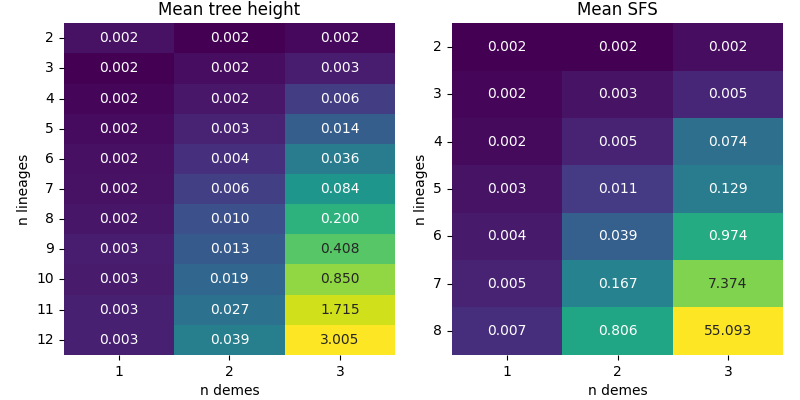
\includegraphics[width=\textwidth]{figures/executions_times}
    \caption{
        Total execution times in seconds for different numbers of lineages and demes.
        The different subplots consider the default and block-counting state spaces with one locus.
        Note that the computation of the SFS required $n$ independent matrix exponentiations, where $n$ is the number of lineages.
    }
    \label{fig:executions_times}
\end{figure}
